\documentclass{llncs}

\usepackage{graphicx}

\usepackage{url}
\urldef{\mailsa}\path|{brendan.annable, mitchell.metcalfe, monica.olejniczak}@uon.edu.au|

% Figures
\usepackage{subfigure}

% Tables
\usepackage[table]{xcolor}
\usepackage{booktabs}
\usepackage{tabularx}

\newcommand{\scarequotes}[1]{`#1'}
\newcommand{\newterm}[1]{{\textit{#1}}}

% References
\usepackage{natbib}
\makeatletter
	% Change natbib numbering style from [#] to #.
	\renewcommand\@biblabel[1]{#1.}
	% Reset bibsection so references appear correctly
	\renewcommand\bibsection%
	{
	  \section*{\refname
		\@mkboth{\MakeUppercase{\refname}}{\MakeUppercase{\refname}}}
	}
\makeatother

% Todo notes
\usepackage{todonotes}
\presetkeys{todonotes}{inline}{}

% Other
\usepackage{hyperref}
\usepackage{float}

\usepackage{pgfplots}
\pgfplotsset{width=\textwidth,compat=1.9}

\begin{document}

	\title{Sphere Detection using Boosted Classifiers}
	\titlerunning{Sphere Detection using Boosted Classifiers}
	\author{Brendan Annable, Mitchell Metcalfe, and Monica Olejniczak}
	\authorrunning{B. Annable, M. Metcalfe, and M. Olejniczak}

	\institute{School of Electrical Engineering and Computer Science \\
				Faculty of Engineering and Built Environment \\
				The University of Newcastle, Callaghan, NSW, 2308, Australia. \\
				\mailsa \\}

	\toctitle{Sphere Detection using Boosted Classifiers}
	\tocauthor{B. Annable, M. Metcalfe, and M. Olejniczak}
	\maketitle

	\begin{abstract}
		Many recent approaches to ball detection attempt to simplify the problem by viewing it as a circle detection problem, or by training a classifier to detect specific balls with known surface texture.
		In this work,%
		% we propose
		a generalisation of the ball detection problem to sphere detection
		is proposed,
		where spherical objects must be detected under unknown lighting and texturing. Approaches used in face detection literature were applied to the problem, namely boosted-classifiers using Haar, HOGS, and LBP features.

		A controlled experiment was performed to test the hypothesis that training a classifier for sphere detection would produce a more robust ball detector. In particular, a detector that does not mis-classify circular, disk-like objects as spheres.

		\todo{discuss results here}

		% We hypothesised that this approach will produce a more robust ball detector. In particular, a detector that does not mis-classify circular, disk-like objects as spheres.


		% We present preliminary results on applying Haar cascade classifiers to the problem, which indicate that classifier performance is extremely sensitive to the training data and settings used.
		\keywords{computer vision, sphere detection, adaboost}
	\end{abstract}

	\section{Related Work} {
	\label{sec:related_work}

		Visually keeping track of a ball is a natural and fundamental aspect of playing soccer, that many human players would not consider to be a skill in itself. However, while it may come naturally to humans, fast and reliable ball tracking has presented a challenge that has attracted much research in the robot soccer community.

		Early attempts at ball detection algorithms used in the international robot soccer competition, RoboCup, simply used histogramming techniques targeted at a specific range of colour intensities to find a coloured ball. As the RoboCup playing field has become less structured over the years, competing teams have needed to account for unpredictable colours and have increasingly implemented methods that detect the shape of the ball as well. \citet{schulz2007ball} used a neural network on subsampled luminance images of the ball to detect the shape of the ball. Recent approaches have focused on detecting the approximately circular shape of the ball in typical images. These include clustering, Hough filters \citep{li2013survey}, and RANSAC \citep{annable2013nubots}.

		Many current ball detection methods make assumptions about the ball or the environment that limit their applicability in a more general case. Methods based on colour classification or similarity can suffer from false positive detections due to other objects having similar colours. These methods may also detect both false positives and false negatives due to unexpected changes in lighting. Methods based on circle or ellipse detection can be effected by false positives due to the presence of disk-like objects in the environment, or due to objects that appear circular when viewed from specific angles.

		To avoid the limitations of methods based on assumptions such as these, we developed a sphere detection method which uses the shading patterns characteristic of spherical objects to classify objects as spheres.

		\citet{nillius2008shading} perform shading based sphere detection using Principal Component Analysis (PCA) with a basis derived analytically from a given Bidirectional Reflectance Distribution Function (BRDF) and assumptions on scene illumination. While this method works well for plain untextured spheres, it is
		not designed to work on spheres with patterns printed on them, like many soccer balls.

		To build a detector that is more robust to differently textured spheres, we investigated the application of techniques popularised in the realm of face detection to the task of sphere detection. We consider this a promising approach, because the 3D features of spheres tend to have similar spatial constraints to facial features in many cases.

		% For simplicity, the scope of this work was limited to the common and important case of detecting balls that are resting on the ground. We also assumed that the sphere is illuminated primarily from above to constrain the likely positions of shadows and specular highlights.

		\citet{masselli2013haar} successfully apply a boosted Haar classifier \citep{viola2001robust} to the problem of ball recognition. They show that the Haar classifier outperformed a more classical approach, based on a Hough transform, in the task of detecting uniformly yellow, green, and white balls.

		\citet{zhang2013novel} used a similar approach, but attempted to detect a wide variety of generic FIFA-style balls. They used extended Haar features \citep{Lienhart2002extended} as weak classifiers. \citet{zhang2013novel} reported improved performance when modified Haar features that used a division operation between their area sums, instead of the usual subtraction, were included. This suggests that exploring alternate weak classifiers could lead to valuable performance improvements.

		\citet{mitri2004fast} applied a Sobel filter and a threshold function to each image as preprocessing steps, passing only the detected edge images to the classifiers. The method learnt Classification and Regression Trees (CARTs) of Haar features instead of directly using Haar features as weak classifiers. Their system performed sufficiently well for ball tracking, but detected other round objects as false positives. It also performed significantly better when a more complex training dataset was applied, which included images under different lighting conditions and environments. We consider it likely that their poor false positive rate was a symptom of ignoring the shading information of the spheres by using only an edge image.

		\citet{treptow2004filter} achieved a much lower false positive rate using Haar features directly, but only trained and tested their detector on a single ball.

		As a result of targeting our approach toward the 3D features that distinguish spheres from objects such as disks, our method is expected to be particularly robust against detecting false positives.

	}

	\section{Training For Sphere Detection} {

		The aim of this project is to create a robust sphere detector that does not detect disk-like objects as false positives.

		We hypothesised that including a larger proportion of disk-like negative images in the training set would increase the precision of the resulting sphere detectors.

		To achieve this, we trained Viola-Jones detector cascades~\citep{viola2001rapid} using each of three different feature types. We tested our hypothesis on each of three commonly used, but different feature types. The feature types used were Extended Haar features~\citep{Lienhart2002extended}, Local Binary Patterns (LBPs)~\citep{liao2007learning}, and Histograms of Oriented Gradients (HoG) features~\citep{dalal2005histograms}.

		The hypothesis was tested through the experiment outlined in Section~\ref{sec:experiment}.

	}

	\section{Experiment} {
	\label{sec:experiment}

		% \todo{Describe the experiment that was performed, including all trials run, all parameters used, and all datasets. Highlight the purpose of the experiment}

		In order to test the hypothesis using the three chosen feature types, the training schemes presented in Table~\ref{tab:training_schemes} were devised.

		\begin{table}
			\centering
			\caption{The training schemes used in the experiment.}
			\label{tab:training_schemes}
			\scalebox{0.8}{
			\begin{tabularx}{1.2\textwidth}{@{}lcccccc@{}}
				\toprule
				\textbf{Name} & \textbf{Set size} & \textbf{Positive \%} & \textbf{Hard Negative \%} & \textbf{NumPos} & \textbf{Simple} & \textbf{Feature type}  \\
				\midrule
					\(scheme_1\) & 2000 & 0.33 & 0     & 138 & Yes & \{Haar, LBP, HOG\} \\ % & 0.75 
					\(scheme_2\) & 2000 & 0.33 & 0.25  & 138 & Yes & \{Haar, LBP, HOG\} \\ % & 0.75 
					\(scheme_3\) & 2000 & 0.33 & 0.25  & 277 & Yes & \{Haar, LBP, HOG\} \\ % & 0.5  
					\(scheme_4\) & 4000 & 0.5  & 0.2   & 420 & No  & \{Haar, LBP, HOG\} \\ % & 0.75 
					\(scheme_5\) & 3500 & 0.5  & 0     & 367 & No  & \{Haar, LBP, HOG\} \\ % & 0.75 
				\bottomrule
			\end{tabularx}
			}
		\end{table}

		Each training scheme specified the size and contents of the dataset, and the training parameters, used to train a classifier.
		The parameter values used in the training schemes were chosen both to test the hypothesis, and to explore the parameter space.
		Five parameters were chosen for the training schemes, and were defined as follows:

		\begin{description}
			\item[Set size:] The total number of samples in the training set.
			\item[Positive \%:] The percentage of samples in the training set that are positive (i.e. that are images of spheres).
			\item[Hard Negative \%:] The percentage of negative samples in the training set that are \scarequotes{hard negatives} (i.e. they are images of disk-like objects, as opposed to miscellaneous background images).
			\item[NumPos:] The number of positive samples shown to each stage of the classifier cascade during training.
			% \todo{Describe the way that NumPos prevents most of the training set from being used.}
			\item[Simple:] 
				Thirteen categories of spheres were chosen from ImageNet \citep{imagenet_cvpr09}.
				The full set of positive samples was drawn from these thirteen categories, listed in Table~\ref{tab:positive_samples}.
				Due to the wide variation in appearance of the spheres in the set, it was considered possible that drawing training samples from the full set while training could cause the trained classifiers to fail to classify any category of sphere with reasonable precision, given the small set sizes used.
				For this reason, a subset of the original thirteen sphere categories were used to create a \newterm{simple training set}.
				The categories selected for the simple set were those that contained mostly images of plain, non-textured spheres, and are listed in Table~\ref{tab:positive_samples_simple}. The two datasets are described in more detail in Section~\ref{sec:dataset}.

				The \newterm{simple} parameter describes whether the simple set of positive samples was used instead of the full set.

				Note that in designing the training schemes, the set size of each training schemes that used the simple training set were restricted to be lower than those that used the full training set, due to the far lesser number of images in the simple set.
		\end{description}

		\subsection{Image Dataset Compilation} {
		\label{sec:dataset}

			ImageNet \citep{imagenet_cvpr09} is an image database organised according to the WordNet hierarchy \citep{fellbaum1998wordnet} that was used as a source of training and testing data. This resource was chosen because it is widely recognised in computer vision, and offers a wide range of images along with associated class and bounding box information. The use of ImageNet has facilitated the collection of many more training samples than would be possible to collect manually within the time-frame of this project.

			% \todo{Add what wordnet is and a reference to why \(24\times24\) is optimised}

			Only images that contained bounding box information were extracted from ImageNet for use as positive training samples. Prior to training, each positive sample was cropped from its original image, using the provided bounding box information, before being  resized to \(24\times24\) pixels and converted to grayscale. An example of this process has been demonstrated in Figure~\ref{fig:samples}.

			% compile / extracted

			\newcommand{\samplefigurewidth}{0.45\textwidth}
			\newcommand{\samplewidth}{0.14\textwidth}
			\newcommand{\sampleheight}{1.5cm}
			\newcommand{\includesample}[1]{\hspace{0.1cm}\includegraphics[width=\samplewidth,height=\sampleheight]{images/training/#1}}

			\begin{figure}
				\centering
				\subfigure[Positive samples.]{%
					% Enclose in shortstack to enable line break.
					\shortstack{%
						% Positive
						\includesample{positive/positive_1}%
						\includesample{positive/positive_2}%
						\includesample{positive/positive_3} \\%
						% Positive thumbnails
						\includesample{positive/positive_1_thumbnail}%
						\includesample{positive/positive_2_thumbnail}%
						\includesample{positive/positive_3_thumbnail}%
					}%
					\label{fig:positive_samples}%
				}%
				\qquad
				\subfigure[Negative samples.]{%
					% Enclose in shortstack to enable line break.
					\shortstack{%
						% Hard negative
						\includesample{hard_negative/hard_negative_1}%
						\includesample{hard_negative/hard_negative_2}%
						\includesample{hard_negative/hard_negative_3} \\%
						% Hard negative thumbnails
						\includesample{hard_negative/hard_negative_1_thumbnail}%
						\includesample{hard_negative/hard_negative_2_thumbnail}%
						\includesample{hard_negative/hard_negative_3_thumbnail}%
					}%
					\label{fig:negative_samples}%
				}%
				\caption{Examples of positive (a) and negative (b) samples used for training. The first row represents the original image, while the second row represents the same samples that have been cropped, resized and converted to grayscale prior to training.}
				\label{fig:samples}
			\end{figure}

			Several WordNet categories (known as \newterm{synsets}) were used to compile the training and test set for this project. Table~\ref{tab:positive_samples} represents the positive samples used in the training set, while Table~\ref{tab:positive_samples_simple} is a subset of these positive samples that were also used for training. The test set was comprised of the categories listed in Table~\ref{tab:test_set}, along with the positive training set samples previously described in Table~\ref{tab:positive_samples}. The imgages for the negative training were drawn from both the list of categories of disk-like objects in Table~\ref{tab:negative_samples}, and the list of categories of background images given in Table~\ref{tab:background_samples}.

			\begin{table}
				\centering
				\caption{ImageNet synsets used for the positive samples in the training set and their associated WordNet identifiers.}
				\label{tab:positive_samples}
				\begin{tabularx}{\textwidth}{@{}lX@{}}
					\toprule
					\textbf{Id} & \textbf{Category} \\
					\midrule
						n02799071 & Baseball \\
						n02802426 & Basketball \\
						n02882301 & Bowling ball, bowl \\
						n03134739 & Croquet ball \\
						n03145719 & Cue ball \\
						n03267113 & Eight ball \\
						n03721047 & Marble \\
						n03742019 & Medicine ball \\
						n03825442 & Ninepin ball, skittle ball \\
						n03942813 & Ping-pong ball \\
						n03982232 & Pool ball \\
						n04409515 & Tennis ball \\
						n04540053 & Volleyball \\
					\bottomrule
				\end{tabularx}
			\end{table}

			\begin{table}
				\centering
				\caption{ImageNet synsets used for the simple positive samples in the training set and their associated WordNet identifiers.}
				\label{tab:positive_samples_simple}
				\begin{tabularx}{\textwidth}{@{}lX@{}}
					\toprule
					\textbf{Id} & \textbf{Category} \\
					\midrule
						n02799071 & Baseball \\
						n03134739 & Croquet ball \\
						n03145719 & Cue ball \\
						n03825442 & Ninepin ball, skittle ball \\
						n03942813 & Ping-pong ball \\
						n03982232 & Pool ball \\
					\bottomrule
				\end{tabularx}
			\end{table}

			\begin{table}
				\centering
				\caption{ImageNet synsets used in the test set, in addition to those used for the set of positive samples, and their associated WordNet identifiers.}
				\label{tab:test_set}
				\begin{tabularx}{\textwidth}{@{}lX@{}}
					\toprule
					\textbf{Id} & \textbf{Category} \\
					\midrule
						n02778669 & Ball \\
						n02779435 & Ball \\
						n02839351 & Billiard ball \\
						n02778669 & Generic sporting equipment balls \\
						n03445777 & Golf ball \\
						n02779435 & Plaything, toy, ball \\
						n04254680 & Soccer ball \\
					\bottomrule
				\end{tabularx}
			\end{table}

			\begin{table}
				\centering
				\caption{ImageNet synsets used for the negative samples in the training set and their associated WordNet identifiers.}
				\label{tab:negative_samples}
				\begin{tabularx}{\textwidth}{@{}lX@{}}
					\toprule
					\textbf{Id} & \textbf{Category} \\
					\midrule
						n03032811 & Circle, round \\
						n13873917 & Circle \\
						n13873502 & Circle \\
					\bottomrule
				\end{tabularx}
			\end{table}

			\begin{table}
				\centering
				\caption{ImageNet synsets used for the background samples in the training set and their associated WordNet identifiers.}
				\label{tab:background_samples}
				\begin{tabularx}{\textwidth}{@{}lX@{}}
					\toprule
					\textbf{Id} & \textbf{Category} \\
					\midrule
						n02782778 & Ballpark, park \\
						n08659446 & Field \\
						n03841666 & Office, business office \\
					\bottomrule
				\end{tabularx}
			\end{table}

		}
	}

	\section{Results} {
	\label{sec:results}

		% \todo{State the results without interpretation, including any basic graphs/tables of the results.}

		% Several Haar cascade classifiers were trained on this datset, using different training parameters, and their performances compared qualatitively by viewing the claissifier output on a small set of test images.

		% The preliminary results obtained are summarised in Table~\ref{tab:results}.
		% These results show that the resulting quality of a classifier is extremely sensitive to the training data and settings used.
		% Some of the classifiers trained show promise, in that they detect balls in some of the images, and appear to detect circular objects in others, but it is clear that most of the supposed detections are false positives.
		% The authors suspect that there are two main reasons for the low classification performance:

		% \begin{itemize}
		% 	\item The set of positive examples is too small and too varied; and
		% 	\item The set of negative examples is poor, in that the images it contains are far too dissimilar from spheres.
		% 		  The use of different ImageNet synsets, such as `n03032811 - Circle, round' into the set of negative samples may improve performance, and will be considered before the final report.
		% \end{itemize}

		The performance of the classifier trained in each trial was evaluated by calculating its \newterm{precision} and \newterm{recall} when run on the test set.
		The results of the classifier training and testing performed for the experiment are summarized in Table~\ref{tab:training_results}, and have been presented graphically in Figure~\ref{fig:trial_comparison_chart_precision}, and Figure~\ref{fig:trial_comparison_chart_recall}.



		% \todo{discuss what recall + precision is}

		

		% \todo{expand, it's rushed}

		% LBP features performed better than HOGS. Increasing the proportion of negative images decreased the hit rate.

		\begin{table}
			\centering
			\caption{Training results for all training schemes.}
			\label{tab:training_results}
			\scalebox{0.75}{
				\begin{tabularx}{1.25\textwidth}{@{}lcccccccc@{}}
					\toprule
					\textbf{Name} & \textbf{Set size} & \textbf{Positive \%} & \textbf{Hard Negative \%} & \textbf{NumPos} & \textbf{Simple} & \textbf{Feature type} & \textbf{Precision \%} & \textbf{Recall \%} \\
					\midrule
						\(haar_1\) & 2000 & 0.33 & 0     & 138 & Yes & HAAR & 42.857 &  9.091 \\
						\(haar_2\) & 2000 & 0.33 & 0.25  & 138 & Yes & HAAR & 53.571 &  6.494 \\
						\(haar_3\) & 2000 & 0.33 & 0.25  & 277 & Yes & HAAR & 36.538 & 16.450 \\
						\(haar_4\) & 4000 & 0.5  & 0.2   & 420 & No  & HAAR & 41.818 & 19.913 \\
						\(haar_5\) & 3500 & 0.5  & 0     & 367 & No  & HAAR & 39.831 & 20.346 \\
						\(lbp_1\)  & 2000 & 0.33 & 0     & 138 & Yes & LBP  & 26.667 &  1.732 \\
						\(lbp_2\)  & 2000 & 0.33 & 0.25  & 138 & Yes & LBP  & 36.842 &  3.030 \\
						\(lbp_3\)  & 2000 & 0.33 & 0.25  & 277 & Yes & LBP  & 36.667 &  4.762 \\
						\(lbp_4\)  & 4000 & 0.5  & 0.2   & 420 & No  & LBP  & 40.000 &  6.061 \\
						\(lbp_5\)  & 3500 & 0.5  & 0     & 367 & No  & LBP  & 38.000 &  8.225 \\
						\(hog_1\)  & 2000 & 0.33 & 0     & 138 & Yes & HOG  & 37.500 &  1.299 \\
						\(hog_2\)  & 2000 & 0.33 & 0.25  & 138 & Yes & HOG  & 50.000 &  0.866 \\
						\(hog_3\)  & 2000 & 0.33 & 0.25  & 277 & Yes & HOG  & 33.333 &  2.597 \\
						\(hog_4\)  & 4000 & 0.5  & 0.2   & 420 & No  & HOG  & 50.000 &  3.030 \\
						\(hog_5\)  & 3500 & 0.5  & 0     & 367 & No  & HOG  & 42.857 &  5.195 \\
					\bottomrule
				\end{tabularx}
			}
		\end{table}

		% Figure~\ref{fig:trial_comparison_chart}

		\newcommand{\plotscheme}[5]{\addplot coordinates {(Scheme 1, #1) (Scheme 2, #2) (Scheme 3, #3) (Scheme 4, #4) (Scheme 5, #5)};}

		\begin{figure}[H]
			\begin{tikzpicture}
				\begin{axis}[
					ybar,
					enlargelimits=0.15,
					legend style={at={(0.5,-0.15)},
					anchor=north,legend columns=-1},
					ylabel={Precision (\%)},
					symbolic x coords={Scheme 1, Scheme 2, Scheme 3, Scheme 4, Scheme 5},
					xtick=data,
					nodes near coords*={\pgfmathprintnumber[fixed,precision=1]\pgfplotspointmeta},
					nodes near coords align={vertical},
				]
				\plotscheme{37.500}{50.000}{33.333}{50.000}{42.857}
				\plotscheme{26.667}{36.842}{36.667}{40.000}{38.000}
				\plotscheme{42.857}{53.571}{36.538}{41.818}{39.831}
				\legend{HOG,LBP,HAAR}
				\end{axis}
			\end{tikzpicture}
			\caption{A column graph comparing each trial scheme with the resulting rate of precision.}
			\label{fig:trial_comparison_chart_precision}
		\end{figure}

 		\begin{figure}[H]
			\begin{tikzpicture}
				\begin{axis}[
					ybar,
					enlargelimits=0.15,
					legend style={at={(0.5,-0.15)},
					anchor=north,legend columns=-1},
					ylabel={Recall (\%)},
					symbolic x coords={Scheme 1, Scheme 2, Scheme 3, Scheme 4, Scheme 5},
					xtick=data,
					nodes near coords*={\pgfmathprintnumber[fixed,precision=1]\pgfplotspointmeta},
					nodes near coords align={vertical},
				]
				\plotscheme{1.299}{0.866}{2.597}{3.030}{5.195}
				\plotscheme{1.732}{3.030}{4.762}{6.061}{8.225}
				\plotscheme{9.091}{6.494}{16.450}{19.913}{20.346}
				\legend{HOG,LBP,HAAR}
				\end{axis}
			\end{tikzpicture}
			\caption{A column graph comparing each trial scheme with the resulting rate of recall.}
			\label{fig:trial_comparison_chart_recall}
		\end{figure}
	}

	\section{Discussion} {

		\todo{Interpret the results and determine whether the hypothesis was correct. Compare the results to other methods. Discuss any additional results not related to the controlled experiment (e.g. performance in practice, the best classifier attained, etc.)}

		A clear trend is visible in Figure~\ref{fig:trial_comparison_chart_recall}, where the recall of the classifiers that used Haar features was much greater than those that used LBPs, which in turn had higher recall than the classifiers using HOG features.

		Figure~\ref{fig:trial_comparison_chart_precision} shows that the Haar classifiers almost always had higher precision than the classifiers using LBP features, although the difference in performance in trials 3--5 may not be significant.
		The classifiers using HOG features also generally had higher precision than those using LBP features, except in \(scheme_3\).

		Based on these observations, the results suggest that Haar features are more appropriate than LBP features for the sphere detection task, as the Haar classifiers had the same are better precision and recall for every training scheme.
		We suggest that this may be 


		% Additionally, recall rate for classifiers of each feature type generally increased with the scheme number. 

		\todo{Results show that Haar is better than LBP.}

		\todo{Rephrase:
			A smaller informal experiment was conducted alongside this project, which involved using a HD webcam to perform live object detection. The webcam was presented with a number of balls with the intention of observing the robustness of the trained sphere detector.
		}
		 This experiment appeared to perform quite well and detected most of the balls in the scene. The sphere detector, however, did not perform well when presented with a highly textured ball as seen in Figure~\ref{fig:fifa_ball}.

		\begin{figure}
			\centering
			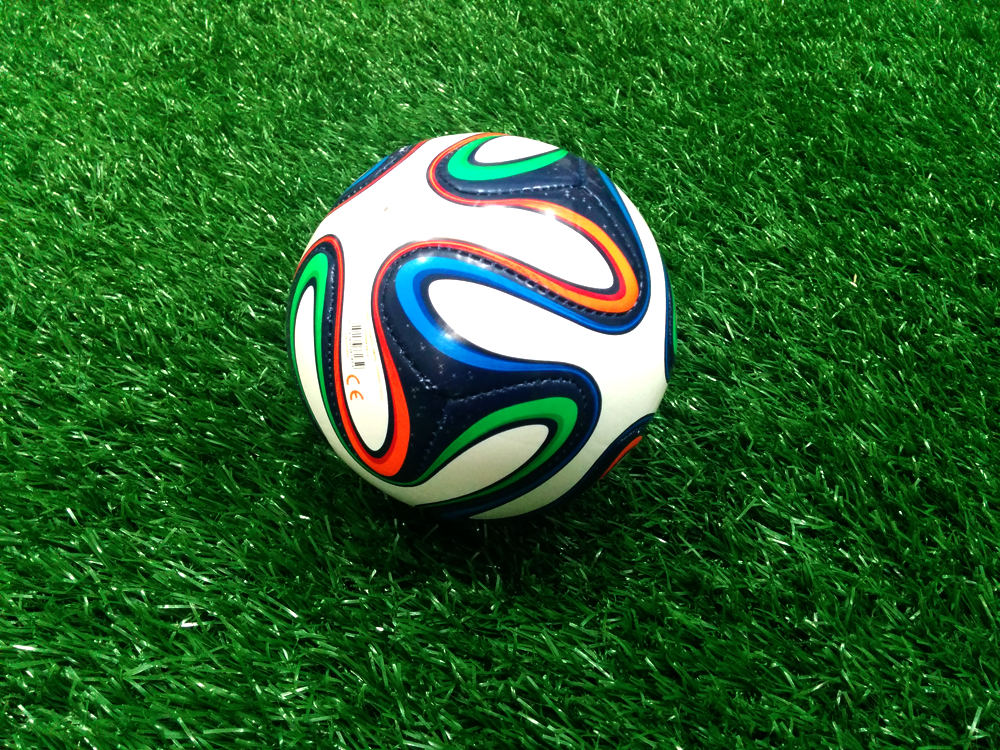
\includegraphics[width=0.5\textwidth]{images/fifa_ball}
			\caption{The FIFA ball that often could not be detected.}
			\label{fig:fifa_ball}
		\end{figure}

		It was also noted that the detector could not detect the balls when the webcam was significantly rotated such that the ball was upside down with respect to the camera. This effect is illustrated in Figure~\ref{fig:rotated_sequence}. This may suggest that the detector must be performing shading based detection and not simply circle detection.

		\todo{note that there is no clear relationship between the number of images used and precision}

% These results indicate that Haar feature-types performed better than HOGS or LBP due to the overall higher precision and recall rate. However, it is clear from this data that HOG has a high precision rate that matches closely to HAAR features. It is interesting to note that using the simple positive training set resulted in a lower rate of recall.

		\newcommand{\includesequence}[1]{\hspace{0.05cm}\includegraphics[width=0.23\textwidth]{images/rotation/#1}}

		\begin{figure}
			\centering
			\includesequence{2}
			\includesequence{25}
			\includesequence{31}
			\includesequence{35} \\
			\vspace{0.1cm}
			\includesequence{39}
			\includesequence{43}
			\includesequence{49}
			\includesequence{53} \\
			\vspace{0.1cm}
			\includesequence{59}
			\includesequence{64}
			\includesequence{69}
			\includesequence{74} \\
			\caption{The sequence of rotated webcam images.}
			\label{fig:rotated_sequence}
		\end{figure}

		\todo{mention disks}

	}

	\section{Conclusion} {
	\label{sec:conclusion}

		\todo{Haar features performed better than HOGS or LBP. LBP features performed better than HOGS. Increasing the proportion of negative images decreased the hit rate.}

		In our future work, we plan to experiment with image preprocessing techniques, to investigate the effect they have on the precision of our sphere detector. These preprocessing techniques should be applied to both the positive and negative samples prior to training and upon classification. We will consider histogram equalisation, gamma intensity correction and high and low pass filtering \citep{gross2003image} as preprocessing techniques in our future work.

	}

	\bibliographystyle{splncsnat}
	\bibliography{references}

\end{document}
